\documentclass[]{article}
\linespread{2}
\usepackage{pdfpages}
\usepackage{lmodern}
\usepackage{amssymb,amsmath}
\usepackage{ifxetex,ifluatex}
\usepackage{fixltx2e} % provides \textsubscript
\ifnum 0\ifxetex 1\fi\ifluatex 1\fi=0 % if pdftex
  \usepackage[T1]{fontenc}
  \usepackage[utf8]{inputenc}
\else % if luatex or xelatex
  \ifxetex
    \usepackage{mathspec}
    \usepackage{xltxtra,xunicode}
  \else
    \usepackage{fontspec}
  \fi
  \defaultfontfeatures{Mapping=tex-text,Scale=MatchLowercase}
  \newcommand{\euro}{€}
\fi
% use upquote if available, for straight quotes in verbatim environments
\IfFileExists{upquote.sty}{\usepackage{upquote}}{}
% use microtype if available
\IfFileExists{microtype.sty}{%
\usepackage{microtype}
\UseMicrotypeSet[protrusion]{basicmath} % disable protrusion for tt fonts
}{}
\usepackage[margin=1in]{geometry}
\ifxetex
  \usepackage[setpagesize=false, % page size defined by xetex
              unicode=false, % unicode breaks when used with xetex
              xetex]{hyperref}
\else
  \usepackage[unicode=true]{hyperref}
\fi
\hypersetup{breaklinks=true,
            bookmarks=true,
            pdfauthor={Zhen Zhang},
            pdftitle={Untitled},
            colorlinks=true,
            citecolor=blue,
            urlcolor=blue,
            linkcolor=magenta,
            pdfborder={0 0 0}}
\urlstyle{same}  % don't use monospace font for urls
\usepackage{natbib}
\bibliographystyle{plainnat}
\usepackage{graphicx,grffile}
\makeatletter
\def\maxwidth{\ifdim\Gin@nat@width>\linewidth\linewidth\else\Gin@nat@width\fi}
\def\maxheight{\ifdim\Gin@nat@height>\textheight\textheight\else\Gin@nat@height\fi}
\makeatother
% Scale images if necessary, so that they will not overflow the page
% margins by default, and it is still possible to overwrite the defaults
% using explicit options in \includegraphics[width, height, ...]{}
\setkeys{Gin}{width=\maxwidth,height=\maxheight,keepaspectratio}
\setlength{\parindent}{0pt}
\setlength{\parskip}{6pt plus 2pt minus 1pt}
\setlength{\emergencystretch}{3em}  % prevent overfull lines
\providecommand{\tightlist}{%
  \setlength{\itemsep}{0pt}\setlength{\parskip}{0pt}}
\setcounter{secnumdepth}{0}

%%% Use protect on footnotes to avoid problems with footnotes in titles
\let\rmarkdownfootnote\footnote%
\def\footnote{\protect\rmarkdownfootnote}

%%% Change title format to be more compact
\usepackage{titling}

% Create subtitle command for use in maketitle
\newcommand{\subtitle}[1]{
  \posttitle{
    \begin{center}\large#1\end{center}
    }
}

\setlength{\droptitle}{-2em}
  \title{Untitled}
  \pretitle{\vspace{\droptitle}\centering\huge}
  \posttitle{\par}
  \author{Zhen Zhang}
  \preauthor{\centering\large\emph}
  \postauthor{\par}
  \predate{\centering\large\emph}
  \postdate{\par}
  \date{January 15, 2016}


% Redefines (sub)paragraphs to behave more like sections
\ifx\paragraph\undefined\else
\let\oldparagraph\paragraph
\renewcommand{\paragraph}[1]{\oldparagraph{#1}\mbox{}}
\fi
\ifx\subparagraph\undefined\else
\let\oldsubparagraph\subparagraph
\renewcommand{\subparagraph}[1]{\oldsubparagraph{#1}\mbox{}}
\fi

\begin{document}

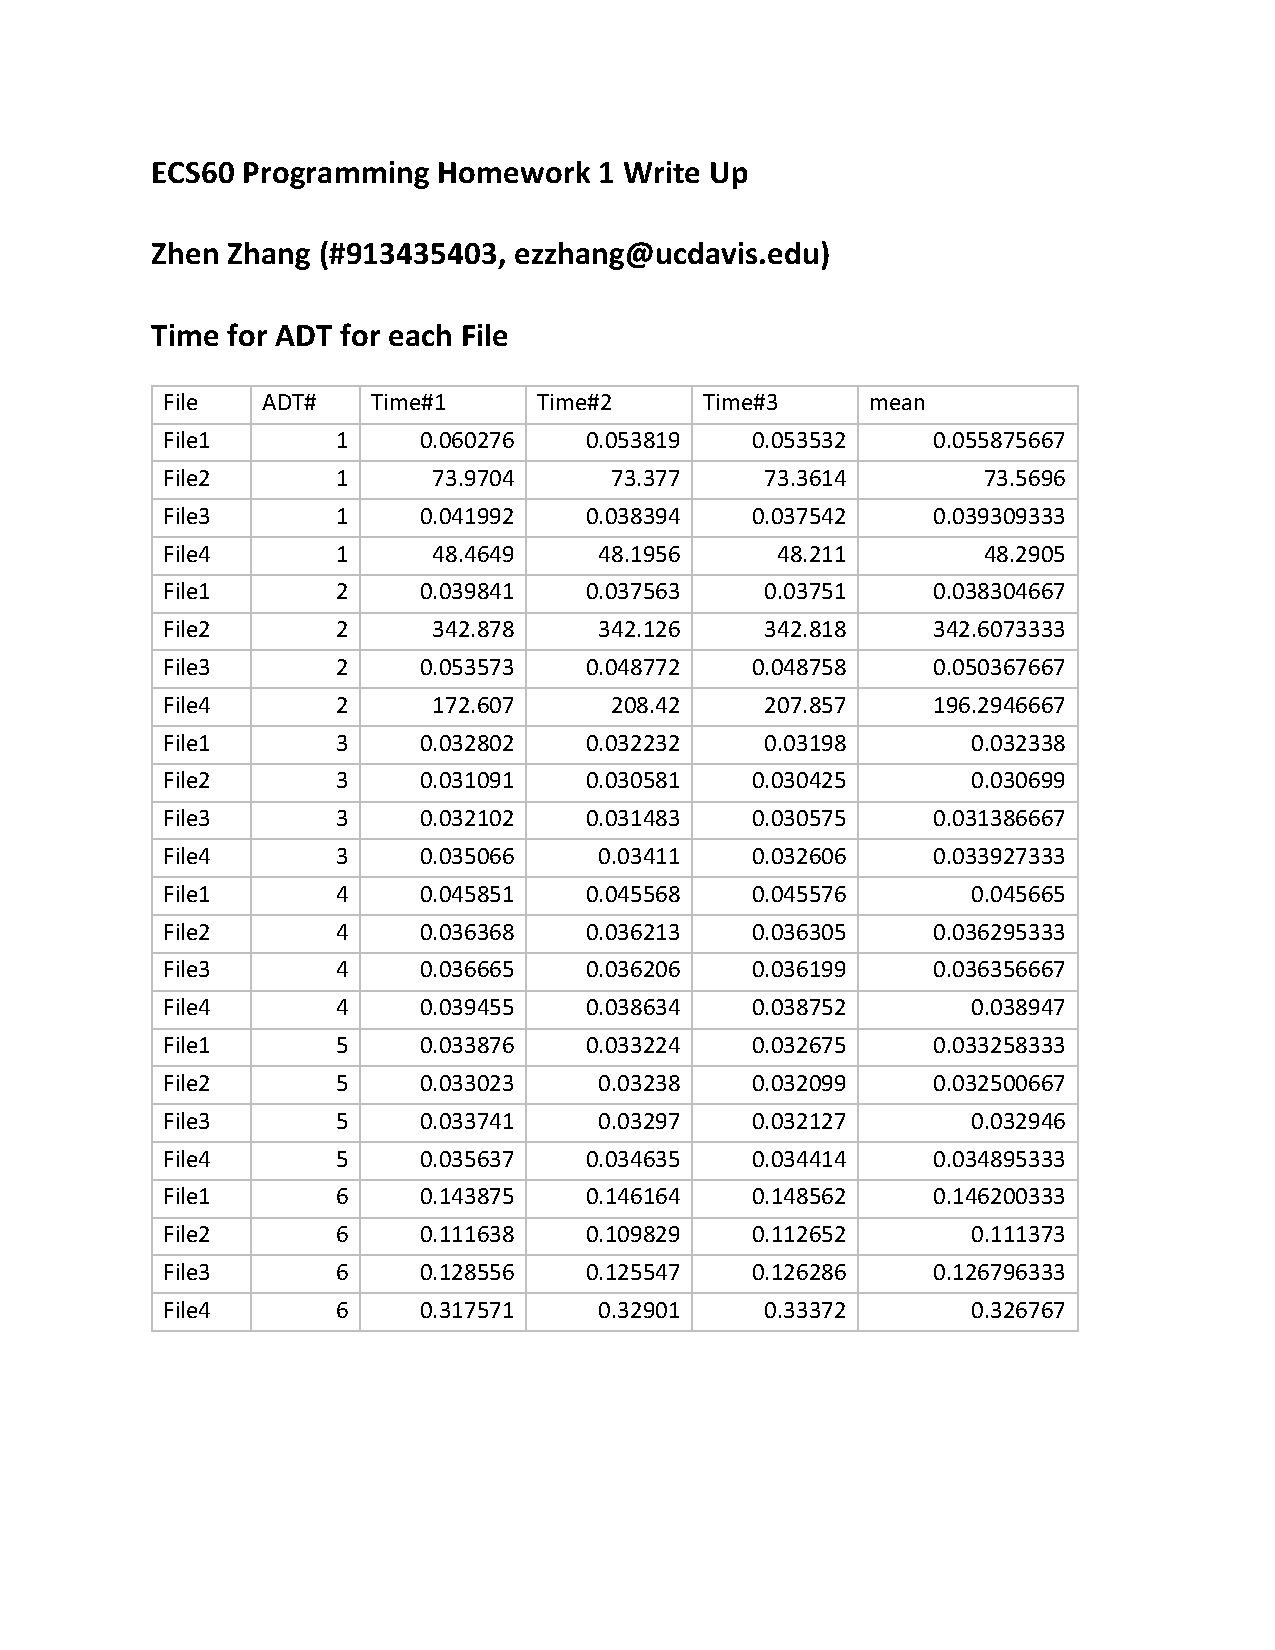
\includegraphics{ECS60p2.pdf}
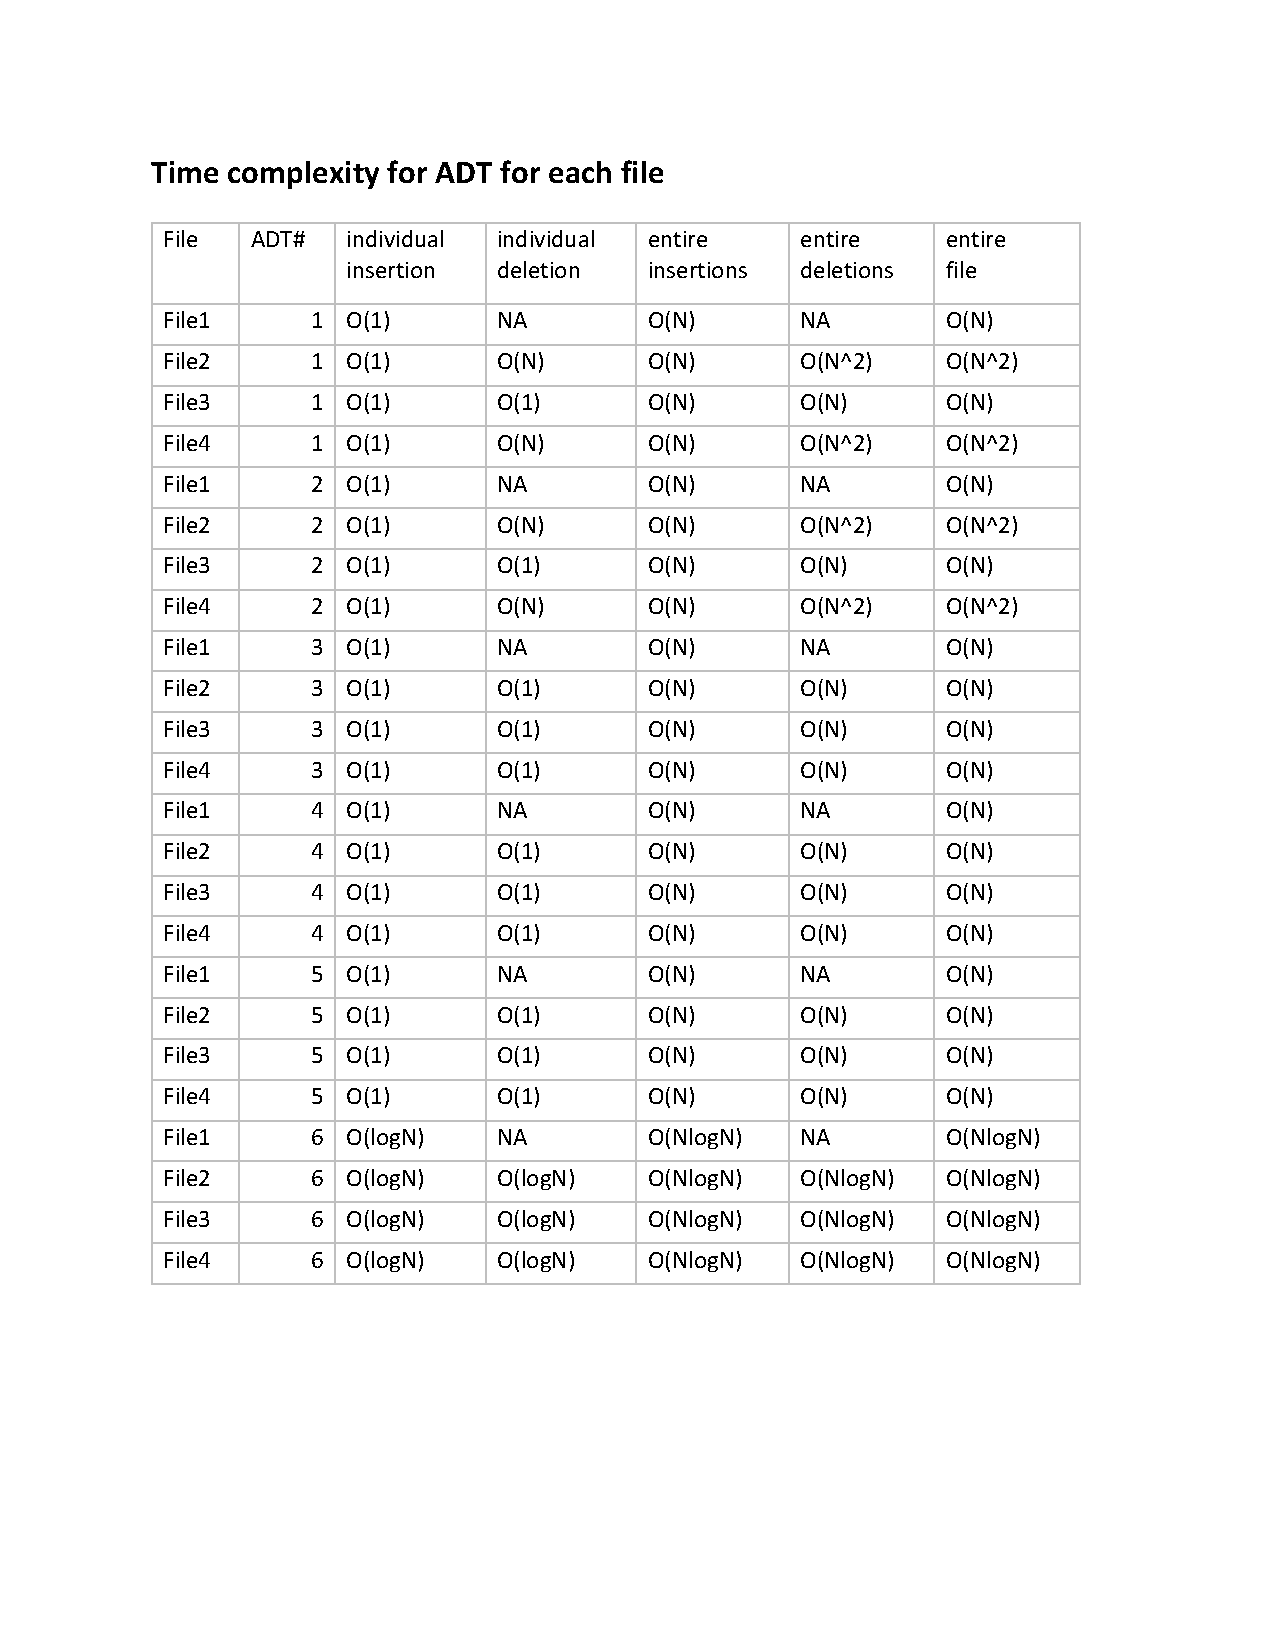
\includegraphics{p2.pdf}

\subsection{Explanation of why ADTs took longer or shorter with
different
files}\label{explanation-of-why-adts-took-longer-or-shorter-with-different-files}

\begin{enumerate}
\def\labelenumi{\arabic{enumi}.}
\item
  LinkedList: For Linked List, File 1 just insert items one by one, but
  for File 2, after inserting, the delete need to be done by delete 1
  first, then 2 second, so on so forth. But the principle of the
  LinkedList is that, when inserting a new node, it pushes the previous
  header and then insert the element as the new header. So at last the
  LinkedList's order 250000, 249999, \ldots{}, 2, 1. Since we can only
  look for the element we want to delete from the header, it takes time
  250000 to find the element 1, and then delete it, so it comes a time
  complexity of O(N). When it comes to File3, the insert is identical,
  but the delete comes as the order of 250000, 249999, \ldots{}, 2, 1,
  so it only takes O(1) each time to do the delete, because the element
  is where the header lies. For the last file, File 4, the time is half
  of File 2, since on average, it will take about N/2 time to find the
  element we want to delete. When comparing File1 with File3, it is just
  comparing insertion time with the delete time. Since insert involves
  creating a ListNode and then let the header pointer points to the new
  Node and the new Node points to the previous Node which is pointed to
  by the header, then give the value to the new Node, while delete only
  involves deleting the ListNode and then let the previous Node points
  to the afterwards Node (Now the find time is only 1 in File3), we know
  insert does more jobs than delete does, and that is why File1 costs
  more time than File3.
\item
  CursorList: The underlying time complexity difference is the same as
  that of LinkedList. The difference is, instead of creating a new Node
  each time, it updates a Node's value and then let the header Node
  points to that one, and the new one to the previous one, so on so
  forth. That means the first inserted element is always the last one to
  get, following the chain. So when deleting in a order of 1, 2,
  \ldots{}., 250000, it will cost O(N) time to the end. This is the
  difference between File2 and 3, in different delete orders. For File4,
  also half the time of that of File2, since the find time is half of
  File2. Since insertion does less operation than deletion, then File3
  costs more time than File1.
\item
  Stack Array, StackList, Queue Array: For the stack, it will not take
  too much time, since when inserting, it will push (enqueue) on the
  top, and when deleting, it will pop (enqueue) the element on the top
  (last), regardless of the value. (the words in parenthesis is for the
  queue array).
\item
  SkipList: For all of them, they have the same time complexity, but the
  result is different. The reason is, for File1, the time is almost
  2Nlog(2N), since the links (number=500000) doubles when compared to
  that of File2 and 3, which is 2*Nlog(2N) (number = 250000). So File1
  costs more time than File2 and 3. For File4, when the order is random,
  it is a little complicated. It has to go thought all the levels to
  find a place to insert, since its place is undetermined, which time is
  at least log(N). Compared with what File1 does, when inserting an
  element that is larger than anyone else in the SkipList, sometimes it
  can get to a very large element directly, omitting some levels, so it
  costs less time. Then in conclusion we know random costs more time
  than ordered elements when inserting into a SkipList.
\end{enumerate}

\subsection{Comparison for ADT}\label{comparison-for-adt}

\begin{enumerate}
\def\labelenumi{\arabic{enumi}.}
\item
  Stack Array, Stack List, Queue Array all have time complexity O(1),
  and Linked List, Cursor List with insertion and delete in reverse
  order have time complexity O(1) as well.
\item
  SkipList have time complexity O(logN), so it needs more time.
\item
  Stack Array, StackList with deletion in ascending order have time
  complexity O(N).
\end{enumerate}

\subsection{The reason for same complexity have different time
value}\label{the-reason-for-same-complexity-have-different-time-value}

\begin{enumerate}
\def\labelenumi{\arabic{enumi}.}
\item
  When comparing the running time of Stack Array, Stack List and Queue
  Array, I noticed that Stack List is implemented on a Linked List while
  Stack Array and Queue Array are implemented on a array. Given a fixed
  size (in this question is 500000), array outperformance Linked List,
  in the sense of random access, no extra storage needed for reference
  and the use of local data caches. So Stack Array and Queue Array will
  almost identical time, and both spend less time than Stack List.
\item
  StackList, Linked List are all Linked Lists, so their time are almost
  the same.
\item
  Now discuss why CursorList is slower than normal LinkedList. In terms
  of deleting in CursorList and LinkedList, the delete operation can be
  decomposed into two parts: first find the node needs to be deleted,
  then delete it. The operation delete spends almost the same time
  between CursorList and LinkedList. Now discuss the find operation. The
  process of find in LinkedList is, use the pointer to find the next,
  check the value using pointer, if it is not the value we are currently
  looking for, use the pointer to find the next one again. It only uses
  pointer to find next. For the CursorList, things become much more
  complicated. This is because CursorList use vector index instead of
  pointer or iterator to extract the element value. To be concrete, we
  use curSorSpace{[}x{]}.element to get the element value, and use
  curSorSpace{[}x{]}.next to get the next index if this value is not we
  are looking for. Since pointer or vector iterator is usually faster
  than vector index, it turns out that CursorList will spend more time
  to do a find operation, which needs more time to delete.
\end{enumerate}

\end{document}
